%%%%%%%%%%%%%%%%%%%%%%%%%%%%%%%%%%%%%%%%%
% fphw Assignment
% LaTeX Template
% Version 1.0 (27/04/2019)
%
% This template originates from:
% https://www.LaTeXTemplates.com
%
% Authors:
% Class by Felipe Portales-Oliva (f.portales.oliva@gmail.com) with template 
% content and modifications by Vel (vel@LaTeXTemplates.com)
%
% Template (this file) License:
% CC BY-NC-SA 3.0 (http://creativecommons.org/licenses/by-nc-sa/3.0/)
%
%%%%%%%%%%%%%%%%%%%%%%%%%%%%%%%%%%%%%%%%%

%----------------------------------------------------------------------------------------
%	PACKAGES AND OTHER DOCUMENT CONFIGURATIONS
%----------------------------------------------------------------------------------------

\documentclass[
	12pt, % Default font size, values between 10pt-12pt are allowed
	%letterpaper, % Uncomment for US letter paper size
	%spanish, % Uncomment for Spanish
]{fphw}

% Template-specific packages
\usepackage[utf8]{inputenc} % Required for inputting international characters
\usepackage[T1]{fontenc} % Output font encoding for international characters
\usepackage{mathpazo} % Use the Palatino font
\usepackage[dvipsnames]{xcolor}
\usepackage{graphicx} % Required for including images
\usepackage{amsmath}
\usepackage{booktabs} % Required for better horizontal rules in tables
\usepackage{listings} % Required for insertion of code
\usepackage{enumerate} % To modify the enumerate environment
\usepackage{ragged2e}
\usepackage{cancel}
\usepackage{MnSymbol,bbding,pifont}
\usepackage{lscape}
\usepackage{array}
\usepackage{float,graphicx}
\usepackage{hyperref}
\newcolumntype{M}{>{$}c<{$}}
%----------------------------------------------------------------------------------------
%	ASSIGNMENT INFORMATION
%----------------------------------------------------------------------------------------

\title{Assignment \#1} % Assignment title

\author{Luis Alberto Ballado Aradias} % Student name

\date{\today} % Due date

\institute{Centro de Investigación y de Estudios Avanzados del IPN \\ Unidad Tamaulipas} % Institute or school name

\class{Tecnologías Computacionales (Sep - Dec 2022)} % Course or class name

\professor{Dr. Edwin Aldana Bobadilla} % Professor or teacher in charge of the assignment

%----------------------------------------------------------------------------------------

\begin{document}

\maketitle % Output the assignment title, created automatically using the information in the custom commands above

%----------------------------------------------------------------------------------------
%	ASSIGNMENT CONTENT
%----------------------------------------------------------------------------------------
\section*{{\color{teal}Climate-neutral container terminal: How does it work?} \url{https://www.youtube.com/watch?v=ApMz1-MK9IQ}}

\begin{itemize}
\item a
\item a
\item a
\item a
\end{itemize}

\newpage
\section*{{\color{BlueViolet}Why learn control systems at all?} \url{https://www.youtube.com/watch?v=oBc_BHxw78s}}

\begin{figure}[H]
  \centering
  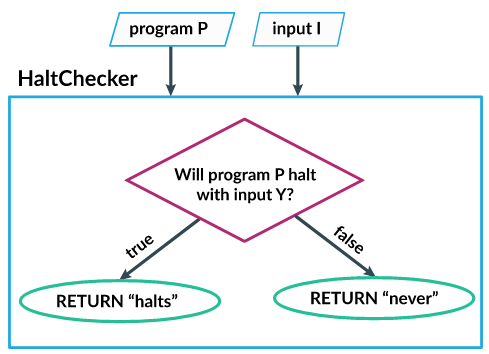
\includegraphics[scale=0.4]{images/halting.png}
\end{figure}

\newpage
\section*{{\color{Apricot}Automation} \url{https://www.youtube.com/watch?v=XJLMW6l303g}}


\begin{itemize}
\item Domino's Form
  \begin{figure}[H]
  \centering
  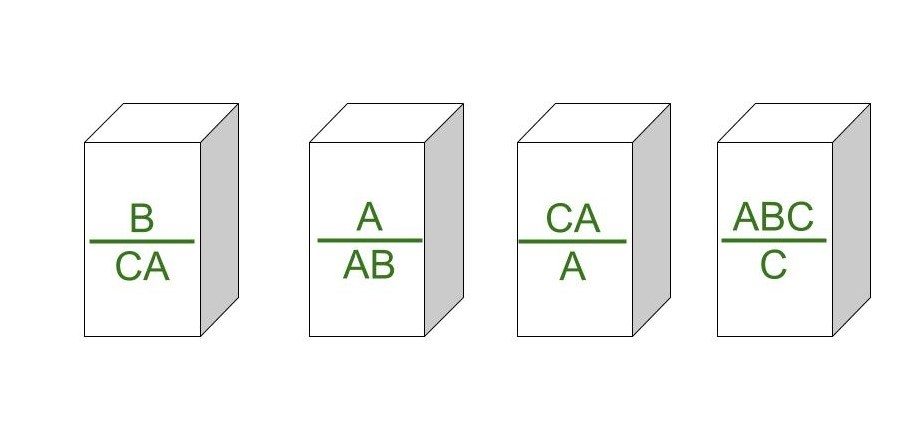
\includegraphics[scale=0.4]{images/dominos.jpg}
\end{figure}
\item Table Form
  \begin{figure}[H]
  \centering
  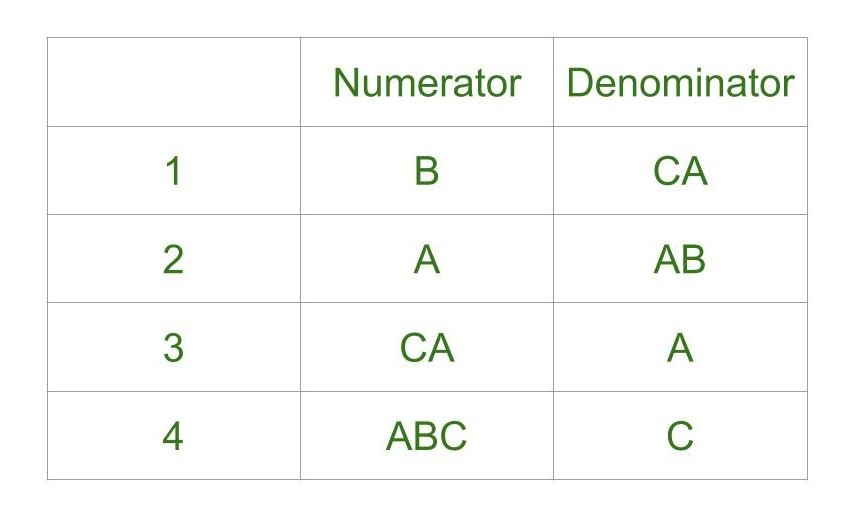
\includegraphics[scale=0.4]{images/table.jpg}
\end{figure}
\end{itemize}

\section*{{\color{Cerulean}Tacoma Bridge} \url{https://www.youtube.com/watch?v=3mclp9QmCGs}}

\begin{figure}[H]
  \centering
  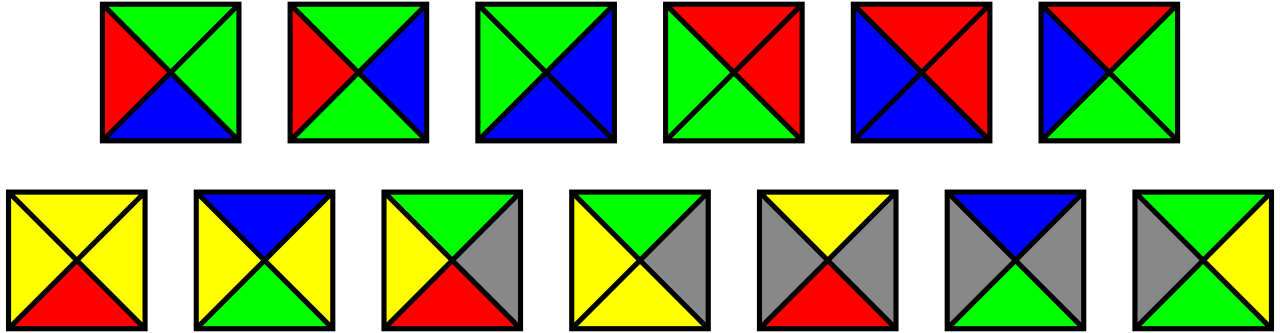
\includegraphics[scale=0.3]{images/wang.png}
\end{figure}

\newpage
\section*{{\color{RoyalPurple}What Control Systems Engineers Do?} \url{https://www.youtube.com/watch?v=ApMz1-MK9IQ&t=610s}}


\begin{enumerate}
\item a
\item s
\item s
\item s
\item s
\end{enumerate}

\newpage
\section*{{\color{RoyalPurple}Control Systems Lectures LTI Systems} \url{https://www.youtube.com/watch?v=3eDDTFcSC_Y&t=377s}}


\begin{enumerate}
\item a
\item s
\item s
\item s
\item s
\end{enumerate}

\newpage
\section*{{\color{RoyalPurple}The Laplace Transform and the Important Role it Plays } \url{https://www.youtube.com/watch?v=VJ9phDRys_I}}


\begin{enumerate}
\item a
\item s
\item s
\item s
\item s
\end{enumerate}

\newpage
\section*{{\color{RoyalPurple}Transfer functions } \url{https://www.youtube.com/watch?v=RJleGwXorUk}}


\begin{enumerate}
\item a
\item s
\item s
\item s
\item s
\end{enumerate}

\end{document}
